\section{Experiments}

\begin{frame}{Experiments}
    We want to see if the each bound is practical, i.e.
    \begin{itemize}
        \item there are minimizers in our classes of interest such that its value is less than 1,
        \item result coincides with train-test split.
    \end{itemize}
    We experiment with neural networks and kernel SVM.
\end{frame}

\begin{frame}{Neural Networks - Adjusting Regularization Parameter}
    Putting Theorem \ref{theorem:decison-theoretic} and \ref{theorem:nn-bound} together and use $\hat{R}_n(F)\le \sqrt{\frac{\pi}{2}} \hat{G}_n(F)$, we have
    $$\EE[\bm{1}(Y\ne f(X)] \le \hat{\EE}_n[\bm{1}(Y\ne f(X)]  + \frac{LB(4\pi \ln k)^{1/2}}{n}\max_{j,j'}\sqrt{\sum_{i=1}^n (x_{ij}-x_{ij'})^2}+ \sqrt{\dfrac{8\ln(2/\delta)}{n}}.$$

    Choose $\delta=0.05$.

    Dataset: subset of Iris with Versicolor $(y=0)$ and Virginica $(y=1)$

    Model: $2$-layer with activation $Tanh$ (L=1).

    Losses (at the end we compute empirical $0-1$ loss)
    $$\texttt{nn.BCEWithLogitsLoss()} + \lambda\sum\limits_{w}|w|\,\,\, \text{(Lasso)}$$
    $$\texttt{nn.BCEWithLogitsLoss()} + \lambda\sum\limits_{w}|w|^2\,\,\, \text{(Ridge)}$$
\end{frame}

\begin{frame}{Neural Networks - Adjusting Regularization Parameter}
    \begin{figure}
        \centering
        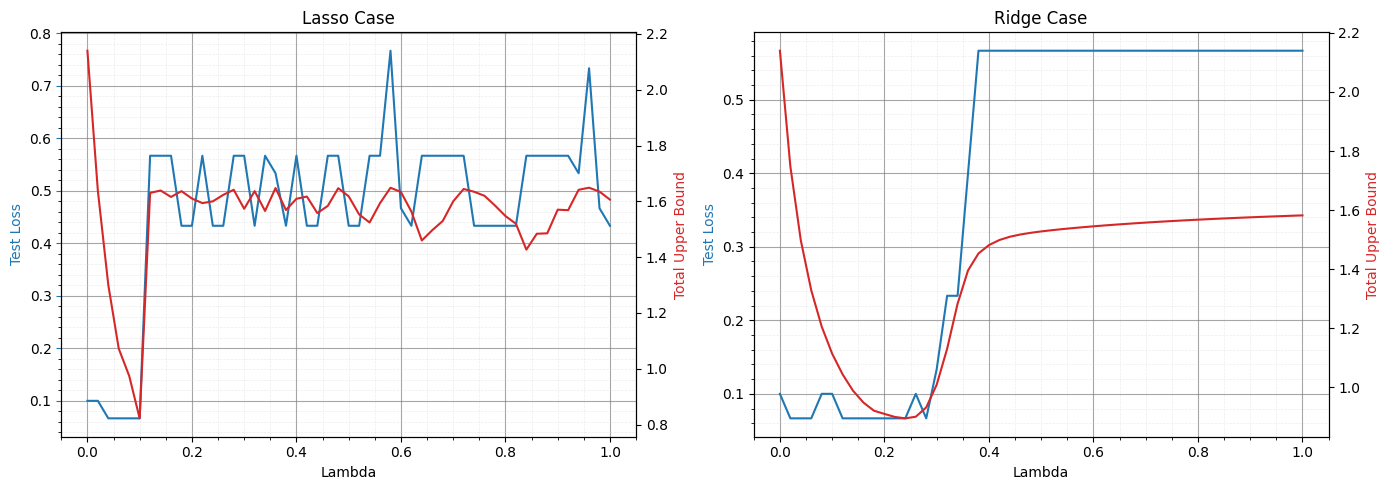
\includegraphics[width=1\linewidth]{nn-lambda.png}
    \end{figure}

    \textbf{Remark.} The bound gives $\lambda=0.1$ in Lasso case and $\lambda=0.25$ in Ridge case, coinciding with the optimal case of test loss.
\end{frame}

\begin{frame}{Neural Networks - Adjusting Depth}
    \begin{myproposition}
        Let $F_2=\left\{\right\}$
    \end{myproposition}
    \begin{myproposition}
        Define a class of $D$-layer networks with $D\ge 2$
        $$F_D = \left\{x\mapsto \sum\limits_{j}w_j\sigma(h_j(x)) : \forall j, h_j\in F_{D-1} \text{ and } \|w\|_1 \le B_D \right\},$$
        where the activation $\sigma$ is $L$-Lipschitz. Then $\hat{G}_n(F_D)\le LB_D \hat{G}_n(F_{D-1})$
    \end{myproposition}
    We want to demonstrate that adjusting depth using the bound is \textit{not} robust.

    We choose a larger dataset \texttt{Breast\_Cancer}, fix a width and continually add layers.
\end{frame}

\begin{frame}{Neural Networks - Adjusting Regularization Parameter}
    The average of $B_1,\ldots, B_D$ is \textit{always} higher than $1$.

    \begin{figure}
        \centering
        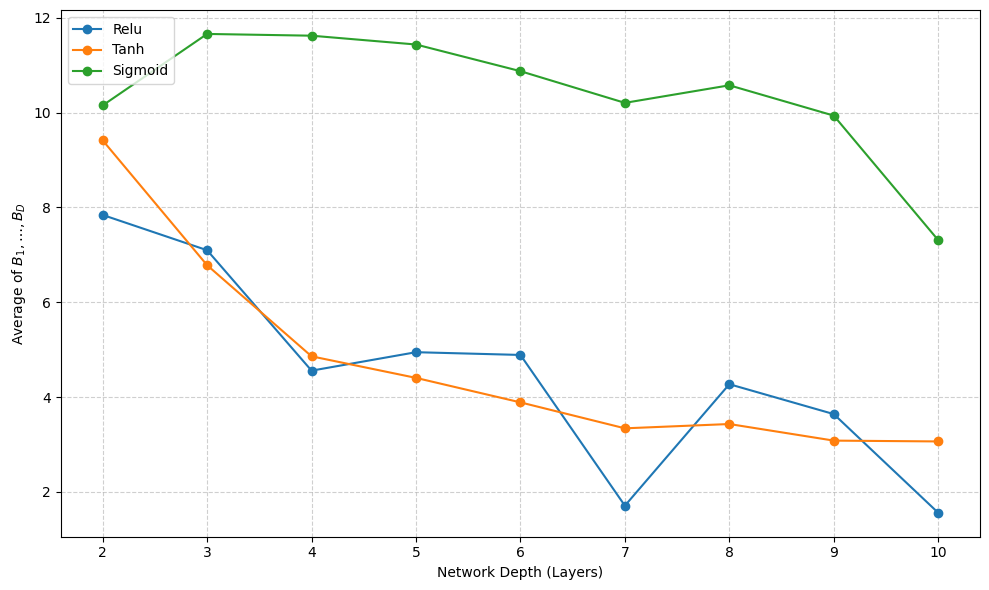
\includegraphics[width=0.7\linewidth]{average_Bd.png}
        \caption{Average of $B_1,\ldots, B_D$ for different $D$'s}
        \label{fig:placeholder}
    \end{figure}
\end{frame}

\begin{frame}{Neural Networks - Adjusting Depth}
    For $Tanh$ and $ReLU$ $(L=1)$, the bound explodes, but the models do not overfit. It fails to capture good models.
    \begin{figure}
        \centering
        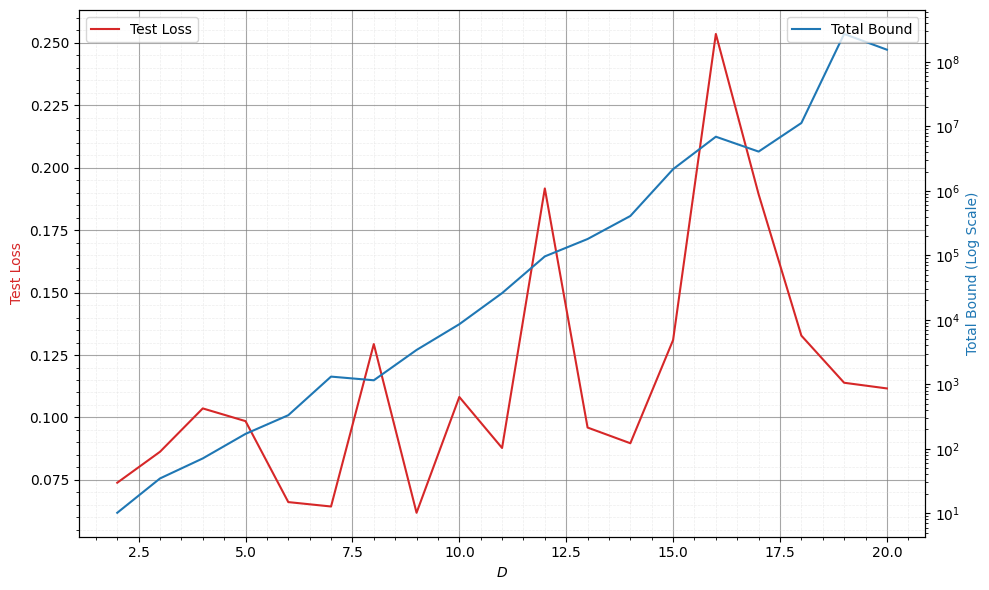
\includegraphics[width=0.75\linewidth]{nn-layers-tanh.png}
    \end{figure}
\end{frame}

\begin{frame}{Neural Networks - Adjusting Depth}
    For $Sigmoid$ $(L=0.25)$, even when the risk bound does not explode, it nominates models having vanishing gradients.

    \begin{figure}
        \centering
        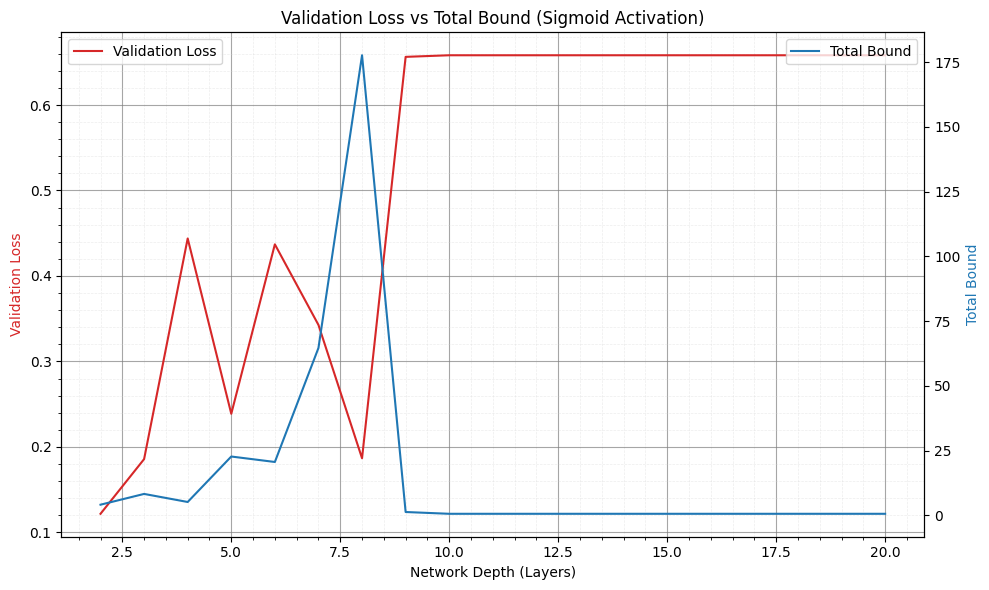
\includegraphics[width=0.75\linewidth]{nn-layers-sigmoid.png}
    \end{figure}

\end{frame}


\begin{frame}{Kernel Methods - Adjusting Regularization Parameter $C$ for SVM}
    Recall the kernelized objective
    $$\max_\alpha \sum_{i=1}^n \alpha_i -\dfrac{1}{2}\sum\limits_{i,j=1}^n \alpha_i \alpha_j y_i y_j K(x_i, x_j), \text{s.t.} \sum_{i=1}^n \alpha_i y_i = 0 \text{ and } 0\le \alpha_i\le C.$$
    \begin{figure}
        \centering
        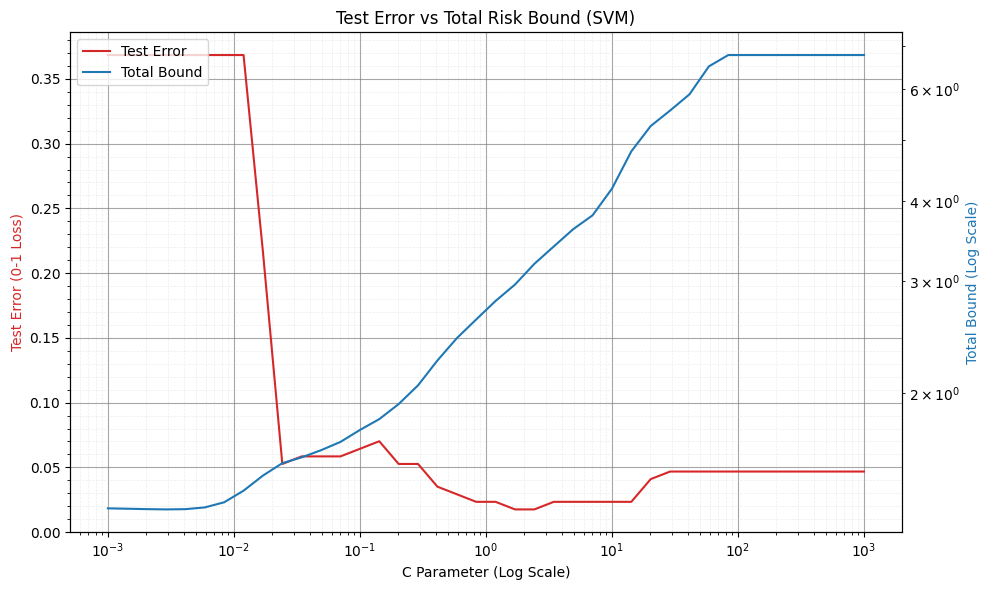
\includegraphics[width=0.7\linewidth]{svm.png}
    \end{figure}

\end{frame}